\chapter{基于情感对的语音情感识别框架}
\label{cha:emo_pair_base_framework}

\section{本章引论}
\label{sec:emo_pair_base_framework_intro}
特征选择作为传统语音情感识别中一个重要的部分,已经吸引了许多的研究者的关注。因为情感是人类的主观感受,想要通过声音中的线索来反应当前说话人的情感状态是一个非常具有挑战性的任务。目前大多数的研究都旨在为所有的情感类别找到一个统一的特征集合,因为这也是通常处理多分类问题的方法,在一个共同的特征集合上构建分类器。但是一些研究结果已经证明与不同的情感相关的声学特征也是不同的,也就是说为所有的情感识别选择相同的特征集合并不是一个很好的方法,为特定的情感选择特定的特征可以取得更好的效果。

基于上述原因,我们认为给不同的情感组合选择相关程度最高的的特征子空间,保证这些情感在这样的特征子空间上具有更高的可分性,是一个比较适合的实现方式。为此,我们提出了一种基于情感对的语音情感识别框架。我们将任意两种不同的情感组成情感对,然后为每一个情感对选择最相关的声学特征子集。这种特征选择方式将在很大程度上缩减需要处理的问题域,因为现在我们将之前需要为多种情感选择特征的问题转换为为两种情感选择特征的问题,剔除了许多无关的干扰特征。当为每一个情感对选择出对应的特征子集之后,我们将在每个特征子集上构建二分类器,这样就将原本的多分类问题转换为多个二分类问题。此时,又存在一个问题,就是最后我们期望的结果是一句话只得到一个识别结果,但现在每个二分类器都会得到一个结果,所以我们还需要再加入一个决策融合的步骤。最简单的决策融合方法就是采用投票策略,将所有二分类器的结果中出现次数最多的那个情感作为最终的识别结果。但投票的策略存在两个缺点,一是会出现票数相同的问题,二是只有和目标情感相关的那些二分类结果才有贡献,其他的二分类结果只会产生干扰。为了避免这两个缺点,我们引入情感空间模型中不同情感之间的距离信息,通过贝叶斯分类器来完成决策融合的步骤,整个系统的流程图如图1所示。

基于层次的语音情感识别框架和我们的设计有着相似的思想,都是期望为不同的情感类别采用不同的特征集合,但是我们的方法效果更好,而且当情感类别发生变化时更容易扩展。此外,由于多个二分类任务之间没有依赖关系,所以更易于并行加速。

本章的剩余部分是这样安排的:首先我们将介绍情感对的定义,基于情感对的特征选择算法,和基于情感对的二分类模型;然后,我们将介绍决策融合的方法,包括基于投票的决策融合和基于情感空间的决策融合;最后,我们将和采用全局特征集合的方法,和基于层次分类的方法进行实验对比。

\begin{figure}[H] % use float package if you want it here
    \centering
    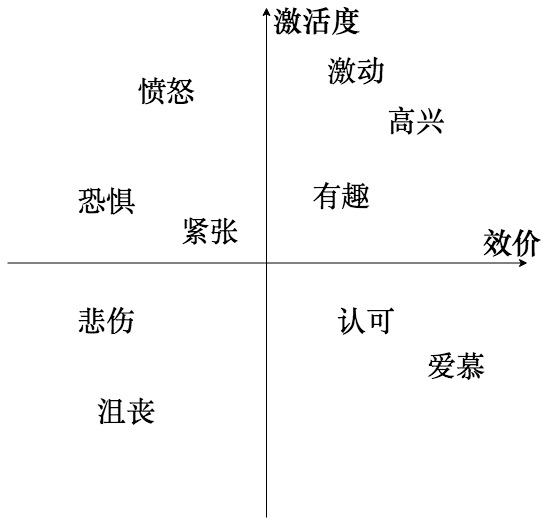
\includegraphics[height=10cm]{myfigures/2dim_space}
    \caption{激活度-效价情感空间模型}
    \label{fig:xfig1}
\end{figure}

\section{情感对}
\label{sec:emo_pair}

\subsection{情感对的定义}
\label{ssec:emo_pair_def}
任意两个不相同的情感组合在一起就被称为情感对,这种思想是源于集成学习(Ensemble Learning)的一些观点。集成学习大致可以分为两种方式,一种被称为引导聚合(Bootstrap Aggregating, Bagging),这种方法利用重采样的方法从整体数据集中采取有放回抽样得到N个数据集,在每个数据集上学习出一个模型,最后的预测结果利用N个模型共同决策得到,例如随机森林(Random Forest)就属于这种方法。总的来说,引导聚合就先训练多个简单的弱分类器,然后通过这些弱分类器组合成一个强分类器。另一种被称为提升方法(Boosting),这种方法是一种可以用来减小监督学习中偏差的机器学习算法。主要也是学习一系列弱分类器,并将其组合成一个强分类器,其中最具代表性的方法是AdaBoost(Adaptive Boosting)算法,这种算法在刚开始训练时对每一个训练样例赋相同的权重,然后对训练集进行多轮迭代训练,每轮训练结束后都对预测错误的那些样例赋以较大的权重,也就是让学习算法以后更注意学错的样本,从而可以得到多个预测模型,最终再以正比于准确率的权重将所有模型的结果组合到一起得到最后的结果。

我们提出的情感对有些类似于引导聚合的思想,我们将为不同的情感对分别选择特征和训练分类器,最后再将所有分类器的结果融合到一起。由于我们只需要为两种情感选择对应的特征,相比于为所有的情感选取相关的特征,这大大减少了干扰特征的引入。和我们有相似思想的还有基于层次的语音情感识别方法,这种方法首先会根据观察设计一棵二叉决策树,在树中的不同节点分别区分不同的情感类别或情感类别组,并且每一个节点的分类器都是单独选择特征集的。情感类别组是指将多种情感分别归属到两个不同的组中,然后将这两个组看做两个类。识别过程是语音从根节点开始进行分类,然后自顶向下沿着路径上的节点依次进行分类,最后到达叶子节点后将会得到一种唯一的情感,整个分类流程如图2所示。但这个方法有两个缺点,第一是整个决策树的结构需要人工来设计,当情感类别或应用场景发生变化时,整个决策树就得重新设计,并不具备通用性。第二是由于整个分类过程是自顶向下的,所以会存在错误累计的问题,就是说如果上一层的分类结果是错误的,这些错分的样本就会沿着路径一直走下去,从而影响下层节点的分类效果。我们基于情感对的方法则可以解决这两个问题,首先情感对的方法不需要任何的人工介入,因为情感对只是将任意两种情感组合到一起,即使需要加入新的情感类别,仅仅只是需要生成新的情感对,之前已经训练好的情感对模型仍然可以使用,这将大大减少训练时间。其次,情感对的方法不存在错误累计问题,因为不同的情感对之间的输入都是独立的,不会相互产生影响。此外,由于不同情感对之间没有依赖关系,所以训练可以并行完成,这将进一步提升训练速度。

\begin{figure}[H] % use float package if you want it here
    \centering
    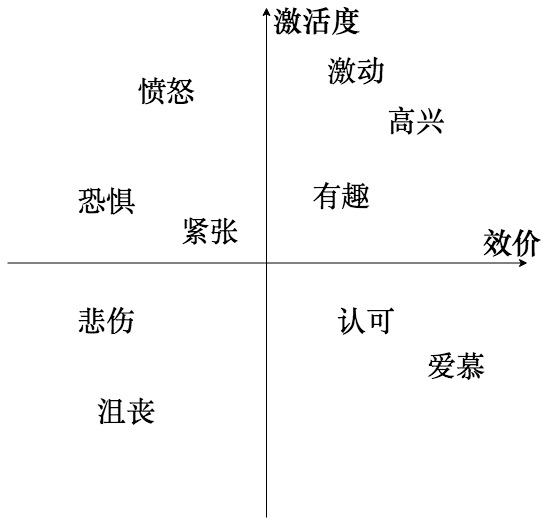
\includegraphics[height=10cm]{myfigures/2dim_space}
    \caption{激活度-效价情感空间模型}
    \label{fig:xfig1}
\end{figure}

下面两小节我们将专门针对基于情感对的声学特征选择算法和二分类模型做出详细的阐述,这两个问题是整个识别框架中最关键的问题。

\subsection{基于情感对的声学特征选择}
\label{ssec:emo_pair_feature_select}
特征选择选择算法有许多,这些算法的目的主要可以分为三个方面:第一是提升模型的预测准确率;第二是筛除无用的冗余特征,减少计算时间;第三是针对于当前的问题域,对于数据提供一个更好的理解。下面将会对特征选择指标,特征选择策略以及基于情感对的特征选择实现这三个方面分别作介绍。

\subsubsection{特征评价指标}
\label{sssec:feature_select_metrics}
对于特征选择算法来说最重要实现选取一种指标来衡量选出的特征的好坏。假设我们有一个含有$m$个样例的数据集$\{\mathbf{x_k}, y_k\}(k=1,...,m)$,每个样例包含$n$个输入特征$x_{k,i}(i=1,...,n)$和一个输出值$y_k(k=1,...,m)$,第$i$个特征的评判指标通过函数$S(i)=f(\{x_{k,i}, y_k\}(k=1,...,m))$来定义。一般来说,我们定义$S(i)$越大的特征和任务目标越相关。为了方便下面的解释,我们再引入一些其他的定义:如果输入向量$\mathbf{x}$被看做来自一个潜在的多变量概率分布$\mathbf{X}$,我们定义$X_i$代表$\mathbf{x}$中第$i$个特征的随机变量。同样,$Y$代表输出值$y$的随机变量。进一步,我们定义$m$维的向量$\mathbf{x_i}$代表数据集中第$i$个特征的所有值,$m$维的向量$\mathbf{y}$代表数据集中所有样本的输出值。

第一种特征评价指标叫做相关系数,我们假设输出$y$是一个连续值,则泊松相关系数被定义为:
\begin{equation}
\label{equ:pearson_cc}
    \Re(i) = \frac{cov(X_i, Y)}{\sqrt{var(X_i)var(Y)}}
\end{equation}
$cov$代表协方差,$var$代表方差。通过统计方法对$\Re(i)$的估计$R(i)$可以表示为:
\begin{equation}
\label{equ:pearson_cc_real}
    R(i) = \frac{\sum_{k=1}^{m}(x_{k,i} - \overline{x_i})(y_k - \overline{y})}{\sqrt{\sum_{k=1}^{m}(x_{k,i} - \overline{x_i})^2}\sum_{k=1}^{m}(y_k - \overline{y})^2}
\end{equation}
符号上面的横线代表对所有的下标$k$求平均值,这个系数也可以看作向量$\mathbf{x_i}$和向量$\mathbf{y}$的余弦值。在线性回归中,评价指标通常是$R(i)$的平方,这样将可以去除负值,用来表示向量$\mathbf{x_i}$和向量$\mathbf{y}$的线性相关性。但是相关系数$R(i)$仅仅可以表示特征和目标之间的线性依赖关系,如果希望可以获取非线性关系,最简单的方法就是对输入进行非线性的处理。例如取平方,开方,取对数等等。

第二种方法是采用单变量分类器,这种方法是将一个特征输入一个分类器中,然后将分类器的预测能力作为衡量指标。通常用来衡量分类器的预测能力的指标是错误率,例如对于二分类问题,错误的识别为正例的比率(Fasle Positive Rate, FPR)和错误识别为负例的比率(False Negative Rate, FNR)都可以被被定义为衡量标准,但通常为了平衡两种错误率,会选择ROC曲线(Receiver Operating Characteristic Curve)下区域的面积,也就是AUC(Area Under Curve)作为衡量的指标。

第三种方法是利用信息学理论中的一些指标,最常使用的是变量和目标之间的互信息量,定义如下:
\begin{equation}
\label{equ:mutual_info}
    I(i) = \int_{x_i}\int_{y}p(x_i, y)log\frac{p(x_i, y)}{p(x_i)p(y)}dydx_i
\end{equation}
其中$p(x_i)$和$p(y)$是$x_i$和$y$的概率密度,$p(x_i, y)$是联合概率密度,$I(i)$是用来衡量变量$x_i$的概率密度和变量$y$的概率密度之间的相关性。连续变量的概率密度$p(x_i)$,$p(y)$和$p(x_i, y)$都是未知的,并且很难从数据集中估计出来。通常在估计连续变量的概率密度时,会先假设变量服从某种已知的概率分布,例如高斯分布,然后通过数据集中变量的统计值来估计这种分布的参数。相对而言,离散变量的概率分布是更容易估计的,因为积分可以通过求和来替代,计算公式如下:
\begin{equation}
\label{equ:mutual_info_discrete}
    I(i) = \sum_{x_i}\sum_{y}P(X=x_i, Y=y)log\frac{P(X=x_i, Y=y)}{P(X=x_i)P(Y=y)}
\end{equation}
公式中的概率可以通过统计不同值出现的的频数。例如,在一个三分类的问题中,输入一共有4个特征,$P(Y=y)$代表类别的先验概率(3种可能),$P(X=x_i)$代表输入特征的分布(4种可能),$P(X=x_i, Y=y)$代表联合概率(12种可能),但是当类别和特征的数量增多时,这种估计也将变得更加困难。

\subsubsection{特征选择策略}
\label{sssec:feature_select_scheme}
上一章我们列举了衡量特征的指标,但是上面的指标主要是针对于单个特征来说的。通常我们选择特征时会选择一个特征子集,并不是说特征子集中所有单个的特征指标最好就代表特征子集是最好的。因为一些研究已经证明,不同特征组合在一起时,相互之间会产生影响。一些评价指标比较低的特征可能刚好补充了其他特征缺失的那一部分信息,一些评价高的特征也有可能和其他特征所包含的信息有重复,所以我们需要通过一些方法来保证能够选择到好的特征子集。特征子集选择的策略大致可以分为两类,一类叫作打包(Wrappers),它是通过预测模型在采用不同特征子集时的预测能力来评价的;另一类叫作过滤(Filters),是通过一些预处理步骤得到特征子集,与预测模型无关,下面分别介绍两类方法。

打包(Wrappers)是一种简单和有效的特征选择策略。在通常情况下,打包(Wrappers)通过预测模型的预测能力来评价特征子集的有效性,所以需要解决的有三个问题:一是如何能够遍历所有的特征子集,二是如何通过预测模型的预测能力指导遍历过程,三是应该选择哪种预测模型。当特征数量不是太多的时候,完全遍历将会被采用。但完全遍历本身是一个NP-hard问题,当特征数量增多时,完全遍历的计算量是难以承受的,一些启发式的遍历算法被提出来降低计算量,期望得到一个近似最佳的结果,例如局部贪心,剪枝搜索,模拟退火,遗传算法等。预测能力则可以使用评价指标中提到的错误率来衡量。预测模型的选择没有太多的理论指导,通常都是根据经验来选取。由于特征选择的过程和选择的预测模型是相关的,因此大多数人通常会将特征选择和模型训练作为一个整体来完成。

过滤(Filters)是另一种特征选择的策略,这种策略不需要预测模型的参与,而是利用一些信息学理论中的指标,仅仅在数据预处理的阶段就能够完成。相比于打包(Wrappers)的策略,一些研究者认为过滤(Filters)的策略有两个主要的优点:一是由于不涉及模型训练,所以处理速度更快;二是这种方法并不针对于某种特定的模型,所以选出的特征更有普适性,在所有的预测模型中都可以使用,不易产生过拟合。这种算法主要利用互信息量这种评价指标,相关的算法比较少,比如马尔科夫毯(Markov Blanket)。

除了上面提到的特征子集选择以外,还有一些特征空间压缩的方法具有相同的效果。特征空间压缩是指将原始的特征空间通过某种函数关系映射到更低维的特征空间,进而提升效果并减少计算量。此外,构建新的特征空间可以帮助我们更好地理解所处理的问题。特征空间压缩的算法有很多,包括聚类方法,线性转换,
小波变换,卷积核等等,下面我们主要介绍聚类和矩阵变换这两类方法。

聚类方法被广泛地用在特征重构上面,这种方法的思想是将一组相似的特征用他们的聚类中心所替代,变成一个新的特征,具体过程如图所示。最流行的算法包括K均值(K-means)和分层聚类。聚类通常是一种无监督的算法,但也可以引入一些监督信息来得到更加有效的特征。假设$\widetilde{X}$是一个代表重构特征的随机变量,$X$代表原有的特征,$Y$代表预测目标。监督式算法的目的是在保证$\widetilde{X}$和$Y$的互信息量$I(\widetilde{X}, Y)$同时,最小化$X$和$\widetilde{X}$的互信息量$I(\widetilde{X}, X)$。这可以通过引入拉格朗日算子$\lambda$来构建全局目标函数:
\begin{equation}
\label{equ:lagrange_multiplier}
    J=I(\widetilde{X}, X) - \lambda I(\widetilde{X}, Y)
\end{equation}
这使得在搜索最大可能的压缩解的同时又可以保证对目标的潜在信息。

\begin{figure}[H] % use float package if you want it here
    \centering
    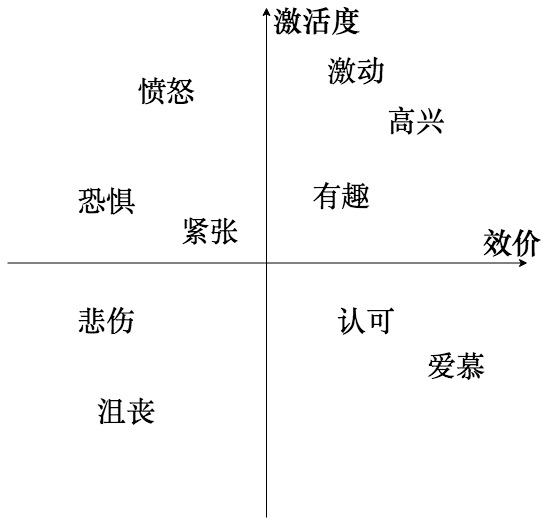
\includegraphics[height=10cm]{myfigures/2dim_space}
    \caption{激活度-效价情感空间模型}
    \label{fig:xfig1}
\end{figure}

矩阵变换是另一种特征空间压缩的方法,常用方法有PCA,SVD,LDA等。这里我们简单解释一下这三个算法的原理,PCA的目的是保证新的特征之间的方差最大,这样可以最大程度保留原始特征的信息。SVD和PCA类似,目标是构成一组由原始特征通过线性组合得到的新特征,并且最大可能保证新的特征保留原始特征的信息,但SVD可以应用在行数和列数不等的矩阵。PCA和SVD都属于无监督的算法,但LDA是一种有监督的算法,它的目标函数是在保证类别内样本的方差尽可能小,类别间样本中心点的距离尽可能大。
 
\subsubsection{基于情感对的特征选择实现}
\label{sssec:emo_pair_feature_select_implement}
在对情感对选择特征子集的时候,我们的目的是从一个大的声学特征集合中选择出一个最能够区分当前情感对中两种情感的特征子集。这里我们采用了打包(Wrappers)的方法,就是将分类器的识别率作为我们筛选特征的指标。首先需要一种遍历算法得到所有可能的特征子集,如果采用全局遍历的话需要耗费太多的时间,所以我们采用了一种启发式的遍历算法序列浮动前向选择算法(Sequential Floating Forward Selection,SFFS)。

SFFS的算法原理是,假设我们选择的特征子集为$S$,初始时$S$为空,每轮迭代从总的特征集合$W$中选出一个子集$A$,使得$A$加入$S$后的的评价函数$J(S)$达到最优,然后再从$S$中选择一个子集$B$,使得$S$剔除$B$后的的评价函数$J(S)$达到最优。经过多轮迭代,评价函数$J(S)$达到我们设定的阈值后算法停止。SFFS被广泛的应用在许多的模式识别任务中,可以在可接受的时间范围内选择出近似最优的特征子集。我们将会为每个情感对都运行SFFS算法得到相关的特征子集,整个特征选择的流程图如下图所示:

\begin{figure}[H] % use float package if you want it here
    \centering
    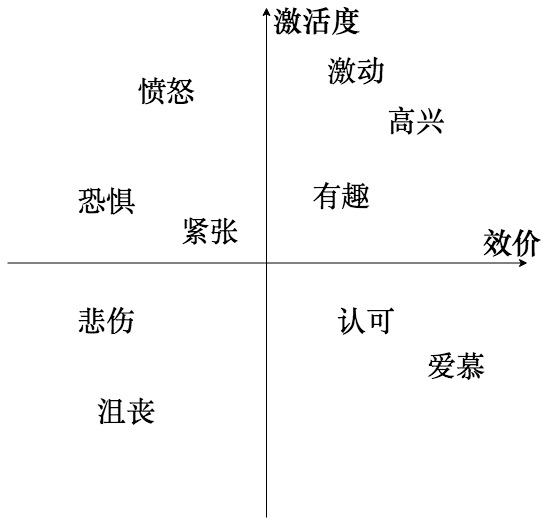
\includegraphics[height=10cm]{myfigures/2dim_space}
    \caption{激活度-效价情感空间模型}
    \label{fig:xfig1}
\end{figure}

\subsection{基于情感对的二分类模型}
\label{ssec:emo_pair_bi_cls}

当我们得到每个情感对相关的声学特征集后,下面的任务就是为每个情感对训练二分类器。二分类器的算法有很多种,在论文中我们采用了两种简单的分类器模型:支持向量机(Support Vector Machine, SVM)和贝叶斯逻辑回归(Bayesian Logistic Regression, BLR)。

SVM是一种二分类模型,它的基本原理是在特征空间中寻找保证使数据点的间隔最大化的分类超平面,如图所示。理想情况下,所有的训练样本都是线性可分的,SVM则可以找到一个完美的分类面将两类数据区分。但大多数情况下,训练样本并不是线性可分的,所以需要其他的一些方法来保证SVM能够正常工作。一般有两种方法:软间隔(Soft Margin)和核函数(Kernel Function)。软边界通过在目标函数中引入松弛变量,从而解决由于个别离群点而导致得到的分类超平面偏移到不好的位置。核函数则是通过将原始数据点映射到给高维的特征空间,使得在低维空间线性不可分的数据点在高维空间变得线性可分。

\begin{figure}[H] % use float package if you want it here
    \centering
    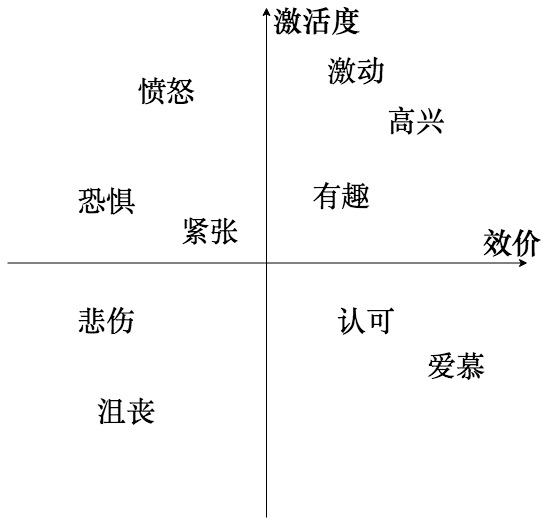
\includegraphics[height=10cm]{myfigures/2dim_space}
    \caption{激活度-效价情感空间模型}
    \label{fig:xfig1}
\end{figure}

 BLR是一种通过假设变量服从某种分布的逻辑回归(Logistic Regression)模型。首先,让我们先回顾下普通的逻辑回归模型,假设我们有特征向量$\phi$,两个类别$C_1$和$C_2$,我们需要建模后验概率$P(C_i|\phi)(i=1,2)$,逻辑回归模型采用下面的公式来建模:
 \begin{equation}
\label{equ:lagrange_multiplier}
    P(C_i|\phi) = \sigma(w^T\phi)
\end{equation}
其中$w$代表我们需要学习的参数,$\sigma$代表sigmoid函数。通过最大似然的算法就可以学习到参数的值。普通的逻辑回归模型都不假设后验概率服从某种分布,这也导致在拟合参数时和训练数据是强相关的,容易出现过拟合的情况。而贝叶斯方法通常都会假设后验概率的分布情况,训练数据通常都是用来估计概率分布的参数,然后再用概率分布去估计类别的概率,这样可以减少过拟合的情况,但是如果数据不服从假设的分布,也会导致训练结果变差。BLR的目的就是将贝叶斯方法的概率分布假设引入逻辑回归的参数估计中,具体来说就是在模型训练时不再精确地估计参数$w$,而是假设参数$w$服从某种分布,然后转而去估计这种分布的参数,这可以通过拉普拉斯近似的方法来实现,具体的细节可以参考[]。通过这种方式就可以有效的避免过拟合的出现,尤其是在训练数据比较少的情况下。

\section{决策融合}
\label{sec:decision_fusion}
在前面一章,我们已经为所有情感对的选择了相关的特征集,并且得到了二分类结果,但我们的目标是只得到唯一的情感类别,所有还需要一个步骤来将这些情感对的结果进行汇总,也就是决策融合。决策融合的算法最早出现在集成学习(Ensemble Learning)领域,因为集成学习通常需要训练多个模型,然后通过决策融合将所有模型的结果整合到一起。决策融合大致可以分为两种:训练型和非训练型。训练型的决策融合就是需要通过训练来建立所有模型的结果和最终结果之间的映射关系,非训练型的决策融合则是通过某些代数规则来将所有模型的结果映射到最终结果。下面会介绍本文中采用的两种决策融合的方法:基于投票的决策融合和基于情感空间的贝叶斯决策融合。

\subsection{基于投票的决策融合}
\label{ssec:voting_decision_fusion}
每一个情感对包含两种情感,二分类器可以得到这两种情感中的一种。假设我们需要识别$M$种情感,则一共可以组成$C_M^2 = \frac{M \times (M - 1)}{2}$个情感对,同样我们也会得到这么多的二分类结果。在所有的二分类结果中,每一种情感出现的次数最多为$M-1$次。基于投票的决策融合就是将所有二分类结果中出现次数最多的那个情感判定为最终的识别结果,因为通常出现次数多代表语音中包含这种情感的信息最多,下这属于一种无需训练的决策融合。下面是算法描述:

\begin{algorithm}[H]
    \caption{投票决策算法}
    \label{alg:voting}
    
    \begin{algorithmic}[1]
        \Require %算法的输入, \hspace*{0.02in}用来控制位置,同时利用 \\ 进行换行
            \Statex $M$: 情感类别的数量 
            \Statex $E = \{e_i, i=1,2,...,M\}$: 情感类别的集合
            \Statex $R = \{r_{e_ie_j}|e_i \neq e_j; r_{e_ie_j}, e_i, e_j \in E\}$: 情感对的二分类结果

        \Ensure %算法的结果输出
            \Statex $f$: 最终识别出的情感类别

        \Statex
        \State  计算$R$中不同情感类别出现的次数$N_e = \{n_{e_i}|e_i \in R\}$ % \State 后写一般语句
        \State  选出$N_e$中次数最多的情感类别,构成候选情感类别集合$C_{max} = \{c_k|c_k \in E; k = 1,2,...K\}$
        \State  $f := c_1$
       \If{$K > 1$} % If 语句,需要和EndIf对应
         \For{$k=2$ to $K$}
                \State $f := r_{fc_k}$
            \EndFor
       \EndIf
        \State \Return $f$
    \end{algorithmic}
\end{algorithm}

投票决策是选取票数最多的情感类别作为最终的结果,但可能会存在出现多个相同最多票数的情感类别的情况。在本文采用投票决策算法中,会将所有最大票数的情感类别放入一个候选集合中,然后依次比较该候选集中两个情感所在情感对的二分类结果,保留胜出的那个情感类别,最后将会只剩下唯一一种情感类别。下面我们将作出形式化的证明:

\begin{proposition}
    投票决策算法在二分类结果正确的情况下一定可以得到正确的情感类别
\end{proposition}
\begin{proof}
    采用和算法~\ref{alg:voting}相同的符号表示,假设$e_i$是目标情感,则可以得到下面的证明过程:
    % \begin{equation*}
    \[
        \begin{aligned}
            R \quad is \quad correct &\Rightarrow n_{e_i} = M - 1 \\
            &\Rightarrow n_{e_j} < M - 1, e_j \in E - \{e_i\} \\
            &\Rightarrow f = e_i
        \end{aligned}
    \]
    % \end{equation*}
\end{proof}

从证明中可以看出当二分类结果是正确的时候,投票决策算法一定可以得到正确的情感类别,但通常我们无法保证所有二分类器的结果都是正确的,这会导致一些情感的票数相同。尽管在算法~\ref{alg:voting}中我们采取了一些策略保证最后可以得到唯一的情感,但是如果同票的几种情感的二分类结果间的胜出关系出现闭环,我们的投票策略同样无法保证得到的一定是最好的识别结果。假设有三种同票的情感$e_1$,$e_2$和$e_3$,$e_1>e_2$代表在$e_1$和$e_2$组成的情感对二分类结果中,$e_1$的概率更高。如果出现$e_1>e_2$,$e_2>e_3$,$e_3>e_1$这种情况,投票策略将无法做出有效的判决。此外,投票策略在判断最终的情感类别时是通过二分类器的结果决策,也就是说只有包含目标情感的那些二分类器才对最终的结果有好的影响,而其他二分类器的结果都不会对识别出正确的情感有好的影响。

\subsection{基于情感空间的贝叶斯决策融合}
\label{emo_space_decision_fusion}
鉴于上一节提到的关于基于投票的决策融合方式存在的问题,我们又提出了一种新的基于情感空间模型的贝叶斯决策融合来避免这些问题。我们在\ref{ssec:continuous_space}节提到过关于维度情感空间的定义,心理学上将情感通过一个笛卡尔空间坐标系来表示,其中每一个坐标轴都表示一种心理学属性,而不同的情感类别会被映射到空间中不同的位置。常用的情感空间模型有二维情感空间(激活度-效价)和三维情感空间(激活度-效价-支配力),本文主要采用三维情感空间模型来描述。假设当前需要识别4种情感:高兴,悲伤,愤怒和中性,这些情感在维度情感空间中的分布大致如下图所示:

\begin{figure}[H] % use float package if you want it here
    \centering
    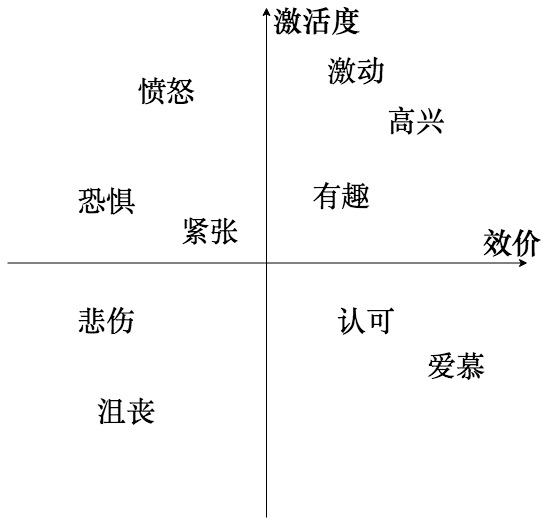
\includegraphics[height=10cm]{myfigures/2dim_space}
    \caption{激活度-效价情感空间模型}
    \label{fig:xfig1}
\end{figure}

从图中我们可以看出不同的情感类别之间的距离并不相同,例如高兴和愤怒的距离明显比高兴和悲伤的距离要小,而这种情感类别之间的距离恰好反映了它们之间的相似程度。回想一下日常生活中,当我们高兴地说话和愤怒地说话时,通常语气都比较急促,声音都比较大,但是当我们悲伤地说话时,声音一般都会比较缓慢而低沉。投票决策有个问题就是不包含目标情感的那些情感对的二分类结果对最后的决策并没有贡献,但现在有了维度情感空间的这种信息,我们可以认为这些不包含目标情感的情感对的二分类结果对最后的决策也是有帮助的。假设目标情感是高兴,对于愤怒-悲伤这个情感对来说,二分类结果是愤怒就更加支持最终的情感类别是高兴,是悲伤的话就更不支持最终的情感类别是高兴,所以二分类结果是愤怒的可能性会更大。这样的支持关系对其他的情感也是适用的,所以如果这种信息能够被有效地运用在决策融合当中,是有助于我们更好地判断最终情感类别的。

对于这种支持关系,需要通过一种数学模型来对其进行量化表示,最为自然的就是想到贝叶斯概率模型,因为这种支持关系可以通过条件概率来建模。假设需要识别的情感类别集合为$E=\{e_i|i=1, 2,...,M\}$,情感对的所有二分类结果为$R = \{r_{e_ie_j}|e_i \neq e_j; r_{e_ie_j}, e_i, e_j \in E\}$。上面关于目标情感为高兴时,对愤怒-悲伤情感对的二分类结果影响程度的例子,通过概率的形式可以表示如下(H:高兴,A:愤怒,S:悲伤):
\begin{equation}
\label{equ:decision_nb_1}
    P(r_{A\_S}=A|H) > P(r_{A\_S}=S|H)
\end{equation}
基于贝叶斯定理,高兴和愤怒-悲伤情感对的二分类结果之间的关系可以被转换为下面的表示:
\begin{equation}
\label{equ:decision_nb_2}
    P(H|r_{A\_S}) = \frac{P(r_{A\_S}|H)P(H)}{P(r_{A\_S})}
\end{equation}
\begin{equation}
\label{equ:decision_nb_3}
    P(H|r_{A\_S}) \propto P(r_{A\_S}|H)
\end{equation}
当$P(H)$和$P(r_{A\_S}$都是先验概率时,通过公式\ref{equ:decision_nb_2}和公式\ref{equ:decision_nb_3},我们可以推导出公式\ref{equ:decision_nb_4}:
\begin{equation}
\label{equ:decision_nb_4}
    P(H|r_{A\_S}=A) > P(H|r_{A\_S}=S)
\end{equation}

为了将这种概率关系推广所有情感对二分类结果的决策融合中,我们通过朴素贝叶斯分类器来建模。目标情感$e_i$的后验概率可以表示如下:
\begin{equation}
\label{equ:decision_nb_5}
    P(e_i|R) = \frac{P(R|e_i)P(e_i)}{P(R)}
\end{equation}
由于不同情感对的二分器分别实在不同的特征集上训练,所以我们可以假设这些二分类器的输出都是条件独立的。这个假设在数学上并不严谨,但这对我们最终的推导结果并没有太大的影响,因为最终的结果只是一个比例关系。基于这种假设,公式\ref{equ:decision_nb_5}可以被表示为下面的公式\ref{equ:decision_nb_6}:
\begin{equation}
\label{equ:decision_nb_6}
    P(e_i|R) = \frac{\prod_{r_{e_je_k} \in R}P(r_{e_je_k}|e_i)P(e_i)}{P(R)}
\end{equation}
类似公式\ref{equ:decision_nb_2}到公式\ref{equ:decision_nb_3}的转换,我们也可以通过公式\ref{equ:decision_nb_6}推导出下面关于目标情感和情感对二分类结果之间的关系:
\begin{equation}
\label{equ:decision_nb_6}
    P(e_i|R) \propto \prod_{r_{e_je_k} \in R}P(r_{e_je_k}|e_i)
\end{equation}

通过上面的概率推导,我们能够得出这样的结论:当采用朴素贝叶斯分类器作决策融合时,不同情感在维度情感空间中的距离信息能够被引入进来。这使得不仅包含目标情感的情感对二分类结果队最终的决策有影响,而且不包含目标情感的情感对二分类结果也可以对最终决策提供辅助信息,进而提升情感识别的准确率。此外,基于贝叶斯的决策融合不存在投票决策中存在的同票问题。在模型训练时,我们将首先得到情感对的二分类结果,再通过朴素贝叶斯分类器建立这些二分类结果和最终目标情感的映射关系。

\section{实验结果及分析}
\label{sec:experiment}

前面几节详细的介绍了我们提出的基于情感对的特征选择和不同的决策融合方法,这两部分共同构成了整个语音情感识别系统,下面我们将通过实验来对比基于情感对的语音情感识别框架和其他语音情感识别框架之间的识别效果。

\subsection{实验设置}
\label{ssec:experiment_setup}

\subsubsection{情感语音数据库}
\label{sssec:speech_database}

在本章中,所有的实验都是基于IEMOCAP情感语音数据库来进行的。在\ref{sec:emo_speech_database}节,我们已经对IEMOCAP数据库做了一个简要的介绍。这是一个人类情感交流相关的数据库,主要被设计用于多模态情感表现研究的,它包括肢体动作,音频和视频,一共有5个部分,每个部分包括10个主题,总共有接近12个小时的数据,语言为英语。每一个部分包含一个不同的对话场景,会有一个男演员和一个女演员分别表演规定好的剧本,以及在一个对话中诱发情感,所有的过程都是在专业的录音棚中进行。至少三个母语为英语的标记员对同一句话标记情感类别,包括高兴,悲伤,中性,愤怒,惊讶,激动,沮丧,厌恶,恐惧这些情感标签。除了离散的情感标签,标记员还需要通过FeelTrace软件标注每个句子在维度情感空间的心理学属性。这个数据库被许多的研究工作采用,因此可以用来与别人的实验结果作对比。在本文中,我们将只采用其中的语音数据,并且只使用那些三个标记员中至少有两个标记为同一种情感标签的句子,这样的句子表达的情感更为清晰。此外,由于数据库中不同情感标签的句子数量不相同,尤其一些情感的句子数量和其他情感相差太多,所以在我们的研究中将只针对愤怒,高兴,悲伤和中性这四种情感。因为这几种情感的语音数据相对较多,同时这也是大多数使用这个数据库的研究所采用的配置。下面的表格\ref{tab:emo_sample_num}列举了属于不同的情感的句子数量。

\begin{table}[htb]
\centering
\begin{minipage}[t]{0.8\linewidth} % 如果想在表格中使用脚注,minipage是个不错的办法
\caption{IEMOCAP数据库中不同情感的句子数量}
\label{tab:emo_sample_num}
    % \begin{tabular}{p{6cm}<{\centering} p{6cm}<{\centering}}
    \begin{tabularx}{\linewidth}{X<{\centering} X<{\centering} X<{\centering} X<{\centering} X<{\centering}}
        \toprule[1.5pt]
        中性 & 愤怒 & 高兴 & 悲伤 & 总计 \\
        \midrule[1pt]
        1708 & 1103 & 595 & 1084 & 4490 \\
        \bottomrule[1.5pt]
    \end{tabularx}
\end{minipage}
\end{table}

本文主要针对于说话人无关的语音情感识别,在实验中我们将不同说话人的数据区分开。数据库由10个演员录制,所以分为10份语音数据,其中1个人的数据作为测试集,1个人的数据作为验证集,剩下8个人的数据作为训练集,并且会采用交叉验证(10-Fold Cross Validation),将10个演员的数据依次作为测试集,最后的准确率是所有测试结果的平均值。交叉验证的方法可以在统计学意义上保证实验结果的有效性和可泛化性,使得模型不会因为数据的改变而产生较大偏差。

\subsubsection{声学特征集合}
\label{sssec:acoustic_feature_set}

表格\ref{tab:acoustic_feature}展示了我们在实验中所采用的声学特征列表和使用的统计函数,这个特征集合被用在Interspeech2009语音情感识别比赛上,因此被许多研究作为基准特征集来使用。我们采用OpenSmile工具包来抽取这些声学特征,特征集合中有16个低级描述子(Low Level Descriptors),包括韵律学特征,谱相关的特征和声音质量特征。由于这些特征都是基于语音帧来抽取,所以将采用统计函数来得到整个句子的特征表示,最终对于每一个句子将会得到384个特征。后面的所有实验都是基于这个特征集合进行的,对于使用全局特征的的模型将会输入所有的384维特征值,而对于选择特征子集的模型将会从这个特征集中选择出最符合当前任务的特征子集。通常会将每个特征子集中特征的数量控制在40-60个,这样设置是为了和之前相关的工作保持一致,从而便于比较。

\begin{table}[htb]
\centering
\begin{minipage}[t]{0.8\linewidth} % 如果想在表格中使用脚注,minipage是个不错的办法
\caption{声学特征列表及其统计函数}
\label{tab:acoustic_feature}
    % \begin{tabular}{p{6cm}<{\centering} p{6cm}<{\centering}}
    \begin{tabularx}{\linewidth}{X<{\centering} X<{\centering}}
        \toprule[1.5pt]
        原始特征类型 & 统计函数 \\
        \midrule[1pt]
        基频(f0) & 均值,标准差,峰值 \\
        均方根能量(rms) & 斜率,最小值,最大值 \\
        过零率(zcr) & 相对位置,范围 \\
        信噪比(hnr) & 二次线性回归系数 \\
        梅尔频率倒谱系数(1-12 mfcc) & 线性回归均方差 \\
        \bottomrule[1.5pt]
    \end{tabularx}
\end{minipage}
\end{table}

在得到每个句子的特征值后,我们采用z-normalization对每一维特征进行正则化,具体做法是计算训练集所有中性样本中每一维特征的均值和标准差,然后将所有样本的对应特征减均值除标准差。这里我们做了一个假设:所有说话人在中性语音上的差异不是很大。通过这种正则化后,可以比较好的消除掉不同说话人的声音特点。

\subsection{实验结果}
\label{ssec:experiment_result}

实验结果主要可以分为两个部分,第一部分主要比较了基于情感对的语音情感识别框架和其他的方法的准确率,并且分析了不同情感的混淆矩阵(Confusion Matrix)的变化;第二部分主要展示当目标情感不同时,所有情感对的二分类结果的分布直方图,从而验证维度情感空间中不同情感的距离信息是能够反应不同情感的相似程度,并且这种相似是可以在模型输出中观测到的。

\subsubsection{准确率对比}
\label{sssec:emo_pair_acc_compare}

首先我们将对比不同方法的加权准确率(Weighted Accuracy, WA)和不加权准确率(Unweighted Accuracy, UA),其中WA的计算方式是用测试集中正确分类的样本数量除以总的样本数量,能够反映分类器模型的整体效果,而UA的计算方式则首先计算出所有情感类别的准确率,然后取平均值,这样的得到的准确率可以反映模型对于不同的情感的识别是否均衡。这两个评价指标在之前许多情感识别相关的比赛中被使用,可以方便和其他人的工作作对比。

在下面的表\ref{tab:acc_emo_pair}中,我们展示了多种语音情感识别方法在上面的实验设置中得到的WA和UA。其中,“全局特征选取”代表对于将语音情感识别建模为多分类任务,为所有的情感选取相同的特征集合;“决策树分层特征选取”代表采用基于决策树的语音情感识别框架,在不同树节点选取不同的特征子集;“情感对特征选取”代表采用基于情感对的语音情感识别框架,为不同的情感对选取不同的特征子集;“+”后面是使用的分类器,“SVM”代表支持向量机,“BLR”代表贝叶斯逻辑回归;对于情感对的方法,还列出了不同的决策融合方法,“投票决策”代表采用投票的决策融合,“贝叶斯决策”代表采用考虑情感空间信息的贝叶斯决策融合。从实验结果中可以看到,基于情感对的框架在不同的分类器上都可以取得比其他框架更好的WA和UA。此外,在情感对的框架中,当我们采用贝叶斯决策方法时,可以取得比采用投票方法更好的效果,这是因为引入不同情感在情感空间中的距离信息有助于在最后决策时更好的判断最终的情感类别。

\begin{table}[htb]
\centering
\begin{minipage}[t]{0.8\linewidth} % 如果想在表格中使用脚注,minipage是个不错的办法
\caption{不同方法的准确率}
\label{tab:acc_emo_pair}
    % \begin{tabular}{p{6cm}<{\centering} p{6cm}<{\centering}}
    \begin{tabularx}{\linewidth}{X<{\centering} X<{\centering} X<{\centering}}
        \toprule[1.5pt]
        模型 & WA & UA \\
        \midrule[1pt]
        全局特征选取 + SVM & 52.41\% & 51.02\% \\
        全局特征选取 + BLR & 53.47\% & 53.55\% \\
        决策树分层特征选取 + SVM & 55.98\% & 58.76\% \\
        决策树分层特征选取 + BLR & 56.38\% & 58.46\% \\
        情感对特征选取 + SVM + 投票决策 & 55.53\% & 58.16\% \\
        情感对特征选取 + BLR + 投票决策 & 56.15\% & 58.54\% \\
        情感对特征选取 + SVM + 贝叶斯决策 & 57.23\% & 62.16\% \\
        情感对特征选取 + BLR + 贝叶斯决策 & \textbf{57.85\%} & \textbf{62.54\%} \\
        \bottomrule[1.5pt]
    \end{tabularx}
\end{minipage}
\end{table}

为了进一步分析不同情感的识别率,我们将展示不同的方法得到的混淆矩阵。为了简单起见,我们将只列出当分类器为BLR时的混淆矩阵,因为SVM得到的结果和BLR是相似的,对于情感对的框架,我们也只展示了贝叶斯决策的结果,因为效果更好。下面的表\ref{tab:cm_global},表\ref{tab:cm_hierarchical}和表\ref{tab:cm_emo_pair}分别是三种不同的框架得到的混淆矩阵,从中我们可以看到基于决策树的框架和基于情感对的框架在所有情感的准确率上都要优于全局选取特征的多分类框架,这证明为不同的情感选取不同的声学特征是有助于提高语音情感识别系统效果的。此外,相对于决策树的框架,我们可以发现情感对的框架在愤怒,高兴,悲伤这三种情感的准确率上都更高,这是因为当我们引入情感空间的距离信息之后,不同情感之间的混淆在决策融合阶段被减轻了。此外,中性情感的准确率并没有发生明显的变化,这可能是因为中性情感在情感空间中和其他情感的距离没有明显的差别,这使得贝叶斯决策并没有产生帮助。这些实验数据证明了我们提出的基于情感对识别框架在非中性情感的识别上是优于基于决策树的框架的。

\begin{table}[htb]
\centering
\begin{minipage}[t]{0.8\linewidth} % 如果想在表格中使用脚注,minipage是个不错的办法
\caption{混淆矩阵(全局特征选取 + BLR)}
\label{tab:cm_global}
    % \begin{tabular}{p{6cm}<{\centering} p{6cm}<{\centering}}
    \begin{tabularx}{\linewidth}{X|X|X|X|X}
        \toprule[1.5pt]
        \diagbox[width=5em,trim=l]{实际}{预测} & 中性 & 愤怒 & 高兴 & 悲伤 \\
        \midrule[1pt]
        中性 & \textbf{52.41\%} & 7.98\% & 16.31\% & 23.30\% \\
        愤怒 & 17.64\% & \textbf{60.55\%} & 18.32\% & 3.49\% \\
        高兴 & 25.32\% & 24.58\% & \textbf{39.28\%} & 10.82\% \\
        悲伤 & 30.12\% & 2.82\% & 5.10\% & \textbf{61.96\%} \\
        \bottomrule[1.5pt]
    \end{tabularx}
\end{minipage}
\end{table}

\begin{table}[htb]
\centering
\begin{minipage}[t]{0.8\linewidth} % 如果想在表格中使用脚注,minipage是个不错的办法
\caption{混淆矩阵(决策树分层特征选取 + BLR)}
\label{tab:cm_hierarchical}
    % \begin{tabular}{p{6cm}<{\centering} p{6cm}<{\centering}}
    \begin{tabularx}{\linewidth}{X|X|X|X|X}
        \toprule[1.5pt]
        \diagbox[width=5em,trim=l]{实际}{预测} & 中性 & 愤怒 & 高兴 & 悲伤 \\
        \midrule[1pt]
        中性 & \textbf{54.51\%} & 6.89\% & 15.20\% & 23.40\% \\
        愤怒 & 16.62\% & \textbf{65.40\%} & 15.26\% & 2.72\% \\
        高兴 & 26.13\% & 19.57\% & \textbf{41.72\%} & 12.58\% \\
        悲伤 & 21.70\% & 2.22\% & 3.88\% & \textbf{72.21\%} \\
        \bottomrule[1.5pt]
    \end{tabularx}
\end{minipage}
\end{table}

\begin{table}[htb]
\centering
\begin{minipage}[t]{0.8\linewidth} % 如果想在表格中使用脚注,minipage是个不错的办法
\caption{混淆矩阵(情感对特征选取 + BLR)}
\label{tab:cm_emo_pair}
    % \begin{tabular}{p{6cm}<{\centering} p{6cm}<{\centering}}
    \begin{tabularx}{\linewidth}{X|X|X|X|X}
        \toprule[1.5pt]
        \diagbox[width=5em,trim=l]{实际}{预测} & 中性 & 愤怒 & 高兴 & 悲伤 \\
        \midrule[1pt]
        中性 & \textbf{53.98\%} & 6.19\% & 12.39\% & 27.43\% \\
        愤怒 & 15.46\% & \textbf{68.04\%} & 12.37\% & 4.12\% \\
        高兴 & 21.94\% & 15.82\% & \textbf{50.51\%} & 11.73\% \\
        悲伤 & 14.93\% & 1.49\% & 5.97\% & \textbf{77.61\%} \\
        \bottomrule[1.5pt]
    \end{tabularx}
\end{minipage}
\end{table}

\subsubsection{情感对二分类结果统计}
\label{sssec:emo_pair_acc_compare}

尽管在识别准确率上显示出考虑情感空间信息的贝叶斯决策方式能够取得更好的结果,但为了进一步证明情感对的二分类结果是符合我们对于情感间的距离能够反映相似度的假设,下面的图1-3将展示出当目标情感不同时,所有二分类结果中不同情感的统计直方图。直方图的计算过程是找到测试集中特定目标情感的所有句子,然后把它们输入所有情感对的二分类器,最后统计这些二分类结果中每一种情感出现的次数,其中横轴代表不同的情感类别,纵轴代表不同情感出现的次数占所有二分类结果的比例,更高的比例表示该情感和目标情感的相似度更高。从图中可以看出,这种比例关系的确和情感空间中不同情感的距离是相关的,例如当目标情感是高兴时,愤怒的比例相对于悲伤的比例更高,而情感空间中也是愤怒和高兴地距离比悲伤和高兴的距离更近。这个统计直方图表明对于情感空间中的距离信息能够反映情感相似度的假设是正确的。

\begin{figure}[H] % use float package if you want it here
    \centering
    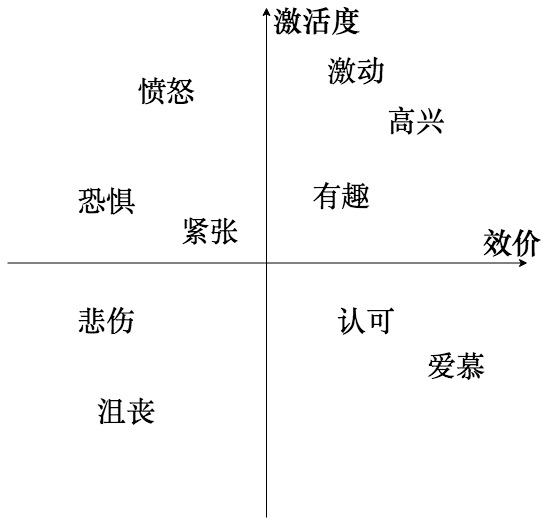
\includegraphics[height=10cm]{myfigures/2dim_space}
    \caption{激活度-效价情感空间模型}
    \label{fig:xfig1}
\end{figure}

\begin{figure}[H] % use float package if you want it here
    \centering
    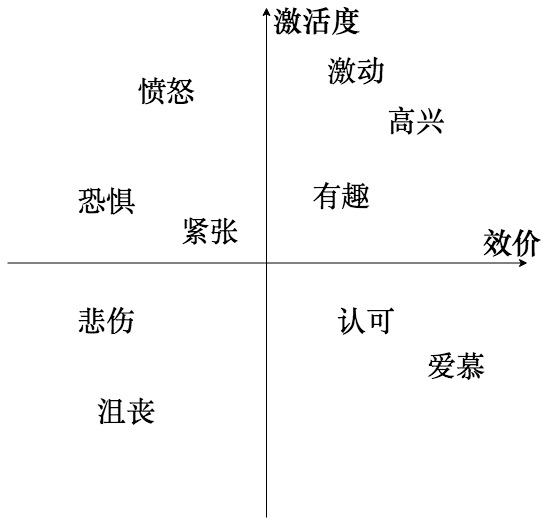
\includegraphics[height=10cm]{myfigures/2dim_space}
    \caption{激活度-效价情感空间模型}
    \label{fig:xfig1}
\end{figure}

\begin{figure}[H] % use float package if you want it here
    \centering
    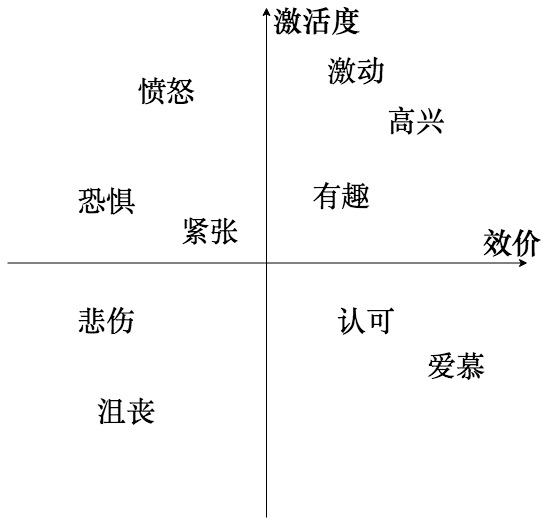
\includegraphics[height=10cm]{myfigures/2dim_space}
    \caption{激活度-效价情感空间模型}
    \label{fig:xfig1}
\end{figure}

\begin{figure}[H] % use float package if you want it here
    \centering
    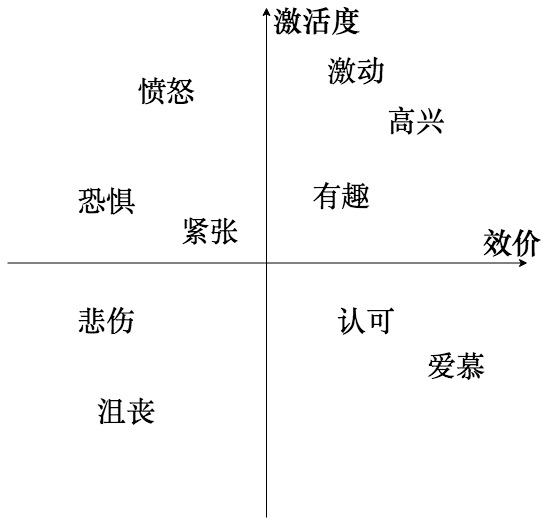
\includegraphics[height=10cm]{myfigures/2dim_space}
    \caption{激活度-效价情感空间模型}
    \label{fig:xfig1}
\end{figure}

\section{本章小结}
\label{sec:emo_pair_summary}

本章我们介绍了基于情感对的语音情感识别框架,通过将任意两种不同的情感组成情感对,并且为每一个情感对从一个大的声学特征集合中挑选出适合的特征子集来训练二分类器,最后再将维度情感空间中不同情感的的距离信息加入到决策融合的过程中,从而避免了投票策略中出现的同票问题和无效情感对的问题。在同样的语音情感数据库IEMOCAP以及同样的实验设置下,相比于传统的全局选取特征的多分类框架和基于决策树的识别框架,基于情感对的识别框架加上贝叶斯决策融合可以达到更好的识别准确率,并且当情感类别发生变化时更方便构建。同时,由于情感对的二分类器训练相互独立,所以可以并行进行。
